\section{Results}
\label{sec:results}

Our results include evaluation of model fit, the Cre-specific connectivity matrices themselves, and retrospective analyses of these matrices for  patterns related to cre-type and source and target regions.

\subsection{Model evaluation}
\label{sec:model_eval}

%Note that this is also the largest evaluation set for 2-stage model, since leave-one-out means of each cre-line may only be computed for lines which are present at least twice in the leaf.

%Clustered source-cell combinations have similar projection patterns.

%In particular, we illustrate which source and cell-type combinations behave similarly, and which target projections tend to co-occur. 

Table \ref{tab:crossvalidation} contains weighted losses from leave-one-out cross-validation of candidate models.
Our EL model generally performs better than the other Nadaraya-Watson estimators that we consider.
For example, the NW Major-WT model is the model from  \citet{Knox2019-ot}.
The EL model combines the good performance of class-specific models like NW Leaf-Cre in regions like Isocortex with the good performance of class-agnostic models in regions like Thalymus.
Additional information on model evaluation, including class and structure specific performance, is given in Appendix \ref{supp_sec:model-evaluation}
In particular, Supplementary Table \ref{tab:loss} contains the sizes of these evaluation sets in each major structure, and Supplementary Section \ref{supp_sec:loss_subsets} contains the structure- and class specific losses.

\begin{table}[H]
\small
\begin{tabular}{lrrrrrrr}
\toprule
& Mean Leaf-Cre & NW Major-Cre& NW Leaf-Cre & NW Leaf &NW Major-WT  & NW Major & EL \\
$\widehat f$ &           Mean & \multicolumn{5}{l}{NW} &     EL \\
$\mathcal D$ & $I_c \cap I_L$ & $I_c \cap I_M$ & $I_c \cap I_L$ & $I_L$ & $I_{wt} \cap I_M$ &  $I_M$ &  $I_L$ \\
\midrule
Isocortex &          0.264 &          0.256 &          0.257 &             0.358 &          0.370 &  0.370 &  \textbf{0.246} \\
OLF       &          0.185 &          0.215 &          0.184 &             \textbf{0.131 }&          0.175 &  0.175 &  0.136 \\
HPF       &          0.176 &          0.335 &          0.170 &             0.201 &          0.235 &  0.235 &  \textbf{0.148} \\
CTXsp     &         \textbf{ 0.758} &          \textbf{0.758} &          \textbf{0.758} &             \textbf{0.758 }&          \textbf{0.758 }&  \textbf{0.758 }&  \textbf{0.758} \\
STR       &          0.131 &         \textbf {0.121} &          0.129 &             0.173 &          0.236 &  0.236 &  0.125 \\
PAL       &          0.220 &          0.223 &          0.220 &             0.339 &          0.324 &  0.324 &  \textbf{0.197} \\
TH        &          0.634 &          0.626 &          0.634 &             0.362 &         \textbf {0.360} &  \textbf{0.360 }&  0.366 \\
HY        &          0.388 &          0.392 &          0.381 &             0.359 &          0.338 &  0.338 &  \textbf{0.331} \\
MB        &          0.213 &          0.232 &          0.201 &             0.276 &          0.285 &  0.285 &  \textbf{0.195} \\
P         &          0.309 &          0.309 &          0.309 &             0.404 &          0.402 &  0.402 &  \textbf{0.306} \\
MY        &          0.261 &          0.340 &          0.261 &             0.188 &         \textbf{ 0.187 }&  \textbf{0.187} &  0.198 \\
CB        &          0.062 &          \textbf{0.061} &          0.062 &             0.067 &          0.111 &  0.111 &  0.068 \\
\bottomrule
\end{tabular}
\label{tab:crossvalidation}
\caption{Losses from leave-one-out cross-validation of candidate models. \textbf{Bold} numbers are best for their major structure.}
\end{table}

%Additional information on model evaluation, including class and structure specific performance, is given in Appendix \ref{supp_sec:model-evaluation}

\newpage

\subsection{Connectivities}

Our main result is the estimation of matrices $\hat {\mathcal C}_v$ representing connections of source structures to target structures for particular cre-lines $v$. 
We exhibit several characteristics of interest, and confirm the detection of several well-established connectivities within our tensor.
Many additional interesting biological processes are visible within this matrix - more than we can report in this paper - and it is our expectation that these will be identified by users of our results.
The connectivity tensor and code to reproduce it are available at \url{https://github.com/AllenInstitute/mouse_connectivity_models/tree/2020}.

\subsubsection{Overall connectivity}

The connectivity matrix for wild-type connectivities from leaf sources to summary structure targets is illustrated in Figure \ref{fig:connectome}.
Several expected biological processes are evident.
For example, intraareal connectivities are clear, as are ipsilateral connections between cortex and thalymus.
The clear intraareal connectivities mirror previous estimates in \citet{Oh2014-kh} and \citet{Knox2019-ot} and descriptive depictions of individual experiments in \citet{Harris2019-mr}.
Compared with \citet{Knox2019-ot}, our more discretized source smoothing and greater number of experiments leads to a significantly more discretized connectivity matrix.
%This is generally expected - for example, different cortical layers have different connectivities.

\newpage

\begin{figure}[H]
\centering
    \subfloat[] {
    \label{fig:full_wt}
   % \raisebox{-.5\height}
    \includegraphics[width = \textwidth]{../../analyses/paper/figures/conn_leafs_0617.png}
    } 
        \newline
       \subfloat[] {
    \label{fig:cortex_wt}
   % \raisebox{-.5\height}
    \includegraphics[width = .5\textwidth]{../../analyses/paper/figures/conn_sum_cortex_0617.png}
    } 
   \caption{Wild-type connectivities.
   \ref{fig:full_wt} Log wild-type connectivity matrix $\log \mathcal {C} (s,t,v_{wt})$.
   \ref{fig:cortex_wt} Log wild-type intracortical connectivity matrix at the summary structure level.}
   \label{fig:connectome}
\end{figure}



\newpage
\subsubsection{Class-specific connectivities}

We have generated $V = 114$ cell-class specific structural connectivities $\mathcal C(v) \in \mathbb R^{S \times T}$.
Exhaustive comparison of this estimated behavior is prohibitive, but we do exhibit several examples of our class specific connectivities conforming to well-known behaviors.
These validation cases are given in Figure \ref{fig:data_ct}.

We begin by plotting subsets of the estimated connectivities in the well-studied VISp and MO regions in Figure \ref{fig:ct_spc}.
The localization of Rbp4-Cre and Ntsr1-Cre injection centroids to layers 5 and 6 respectively is evident (see also Supplemental Figure \ref{fig:iso_count}). 
These layers project to their expected targets \citet{Jeong2016-dc}.
In VISp, the Ntsr1-Cre line strongly targets the thalymic LP nuclei, and in MO, layer 5 projects to anterior basolateral amygdala (BLA) and capsular central amygdala (CEA), while layer 6 does not.

Figure \ref{fig:ct_clust} shows a collection of connectivity strengths generated using cre-specific models for wild-type, Cux2, Ntsr1, Rbp4, and Tlx3 cre-lines from visual signal processing leafs in the cortex to cortical and thalymic nucleii.
This shows that cell-class has a dominating effect on projection in certain regions.
We use heirarchical clustering to sort source structure/cell-class combinations by the similarity of their structural projections, and sort target structures by the structures from which they receive projections.
Examining the former, we can see that the Ntsr1 Cre-line distinctly projects to thalymic nucleii, regardless of summary structure.
This contrasts with the tendency of other cell classes to project intracortically in a manner determined by the source structure.
Similarly, layer 6 targets are not strongly projected to by any of the displayed Cre-lines.
There are too many targeted summary structures to plot here, but we expect that the source profile of each target clusters by structure.

\newpage

\begin{figure}[H]
\subfloat[]{
\label{fig:ct_spc}
    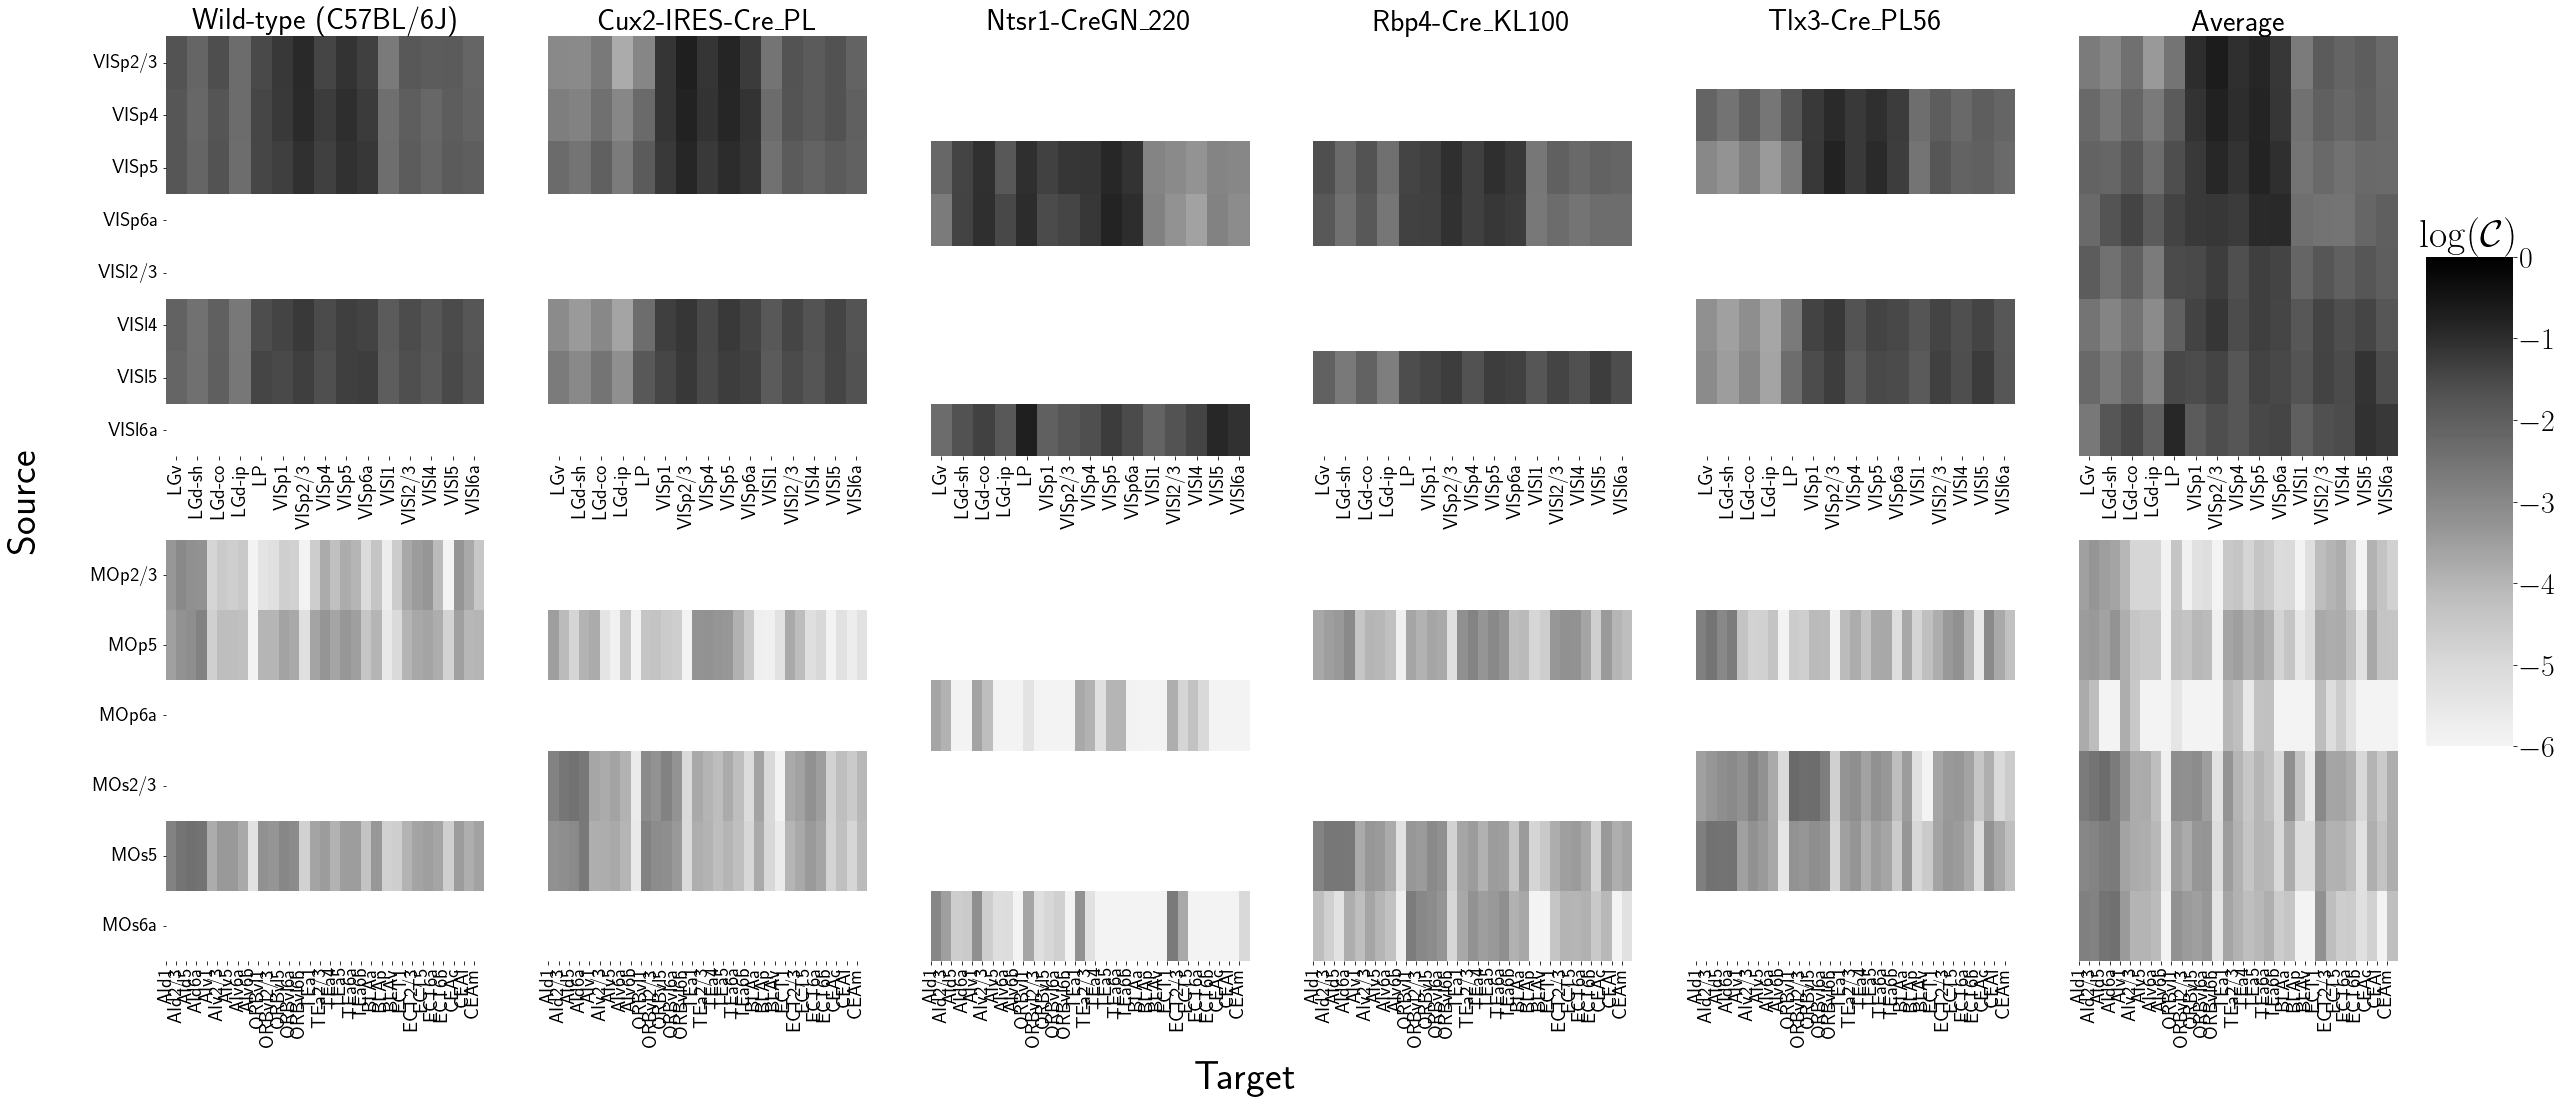
\includegraphics[width=.8\textwidth]{../../analyses/paper/figures/visp_mo_0615.png} 
    }
    \newline
 \subfloat[]{
 \label{fig:ct_clust}
    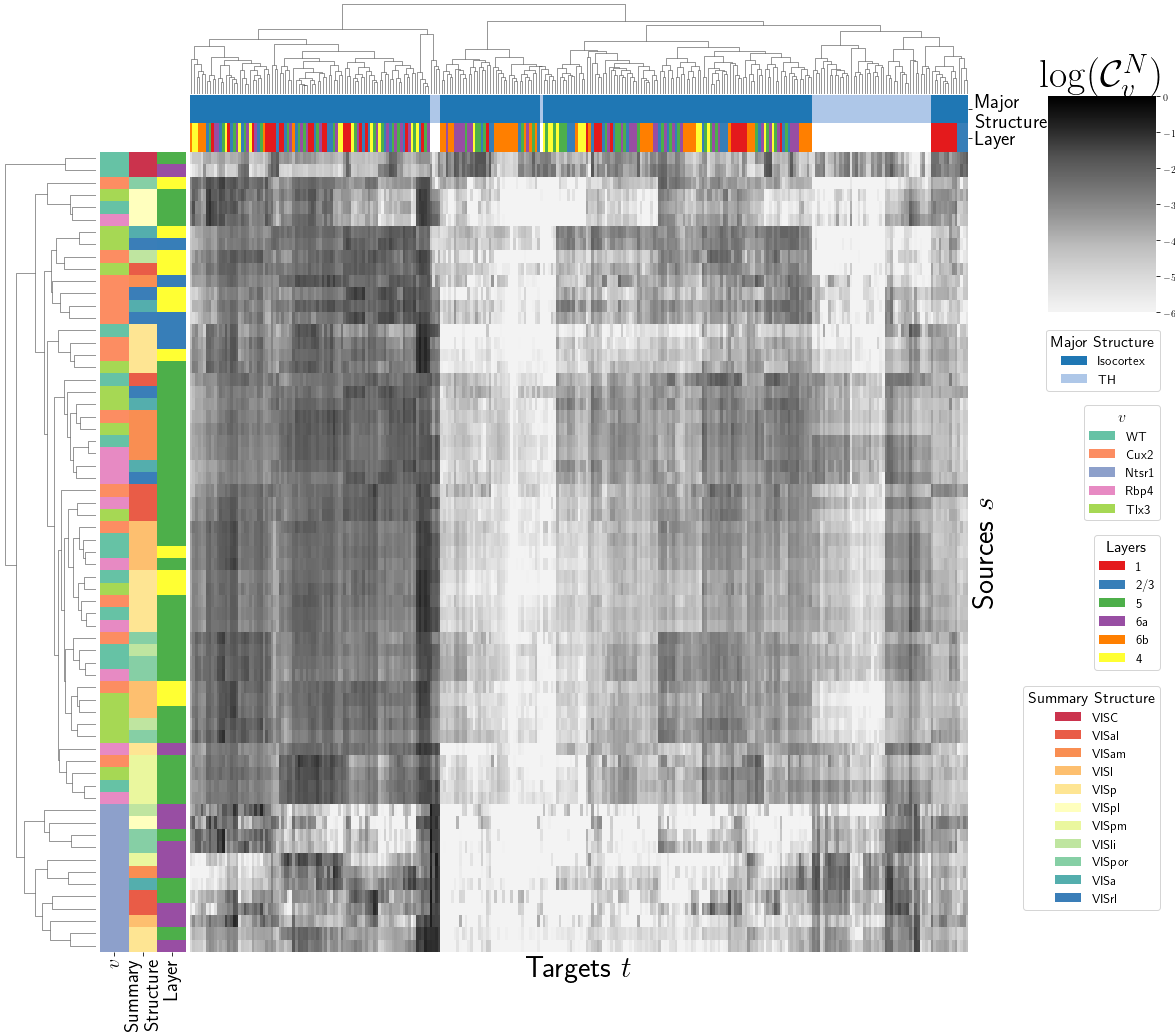
\includegraphics[width=.8\textwidth]{../../analyses/paper/figures/heirarchical.png}
    }
    
    \caption{ Cell-class and layer specific connectivities from VISp and MO.
    		This figure shows a preselected subset of putatively interesting connectivities from VISp and MO.
    		\ref{fig:data_ct}
		Heirarchical clustering of connectivity strengths from visual signal processing cell-types to cortical and thalymic targets.
		Cre-line, summary structure, and layer are labelled on the sources.
		Major brain division and layer are labelled on the targets.
		Note that sources/cre combinations are only included if there is at least one experiment of that cre-line in that particular leaf.}
\label{fig:data_ct}
\end{figure}

\newpage

\subsection{Connectivity Analyses}

Each structural connectivity matrix is a high-dimensional representation of relatively few biological processes.
As discussed in \citet{Knox2019-ot}, one of the most basic processes underlying the observed connectivity is the tendency of each source region to predominantly project to proximal regions.
For example, the heatmap in \ref{fig:dist_bw_str} shows intraregion distances clearly contains an overall pattern reminscent of the connectivity matrix in \ref{fig:connectome}.
These connections are biologically meaningful, but also unsurprising, and their relative strength biases learned latent coordinate representations away from long-range structures.
For this reason, we establish a $1500 \mu m$ 'distal' threshold within which to exclude connections for our analysis.

Perhaps more interestingly in our setting, certain cell-types and layers have a characteristic connectivity pattern.
We therefore perform non-negative matrix factorization on distal wild-type connectivities to estimate these characteristic patterns in a probabilistic way.
This decomposes the remaining censored connectivity matrix into a relatively small number of distinct signals.
These signals are plotted in Figure \ref{fig:nmf_results}, and technical details and intermediate results are given in Supplemental Sections \ref{supp_sec:matrix_factor_methods} and \ref{supp_sec:matrix_factor_results}, respectively.

The plotted decomposition shows that these underlying connectivity archetypes correspond strongly to major brain division.
However, certain components that predominantly represent connectivity from a given major brain division may also be accessed from other areas.
For example, the IP and FN regions of CB are strongly associated in \ref{fig:W} with the component projecting to MY in \ref{fig:H}.
%The overall wild-type connectivity strength matrix also displays an underlying modelable structure.

%This relationship is plotted in \ref{fig:nmf} b), showing that there exists substantial variability that would be impossible to model with low-error in a univariate model, even using the diffusion model suggested in \citet{Knox2019-ot}.
%We then apply non-negative matrix factorization (NMF) to 


%, and apply an unsupervised cross-validation method to select the optimum number of signals %\skcomment{Percent error... show reconstruction? log scale?}.

\newpage

\begin{figure}[H]
\begin{tabular}[t]{c}
\subfloat[]{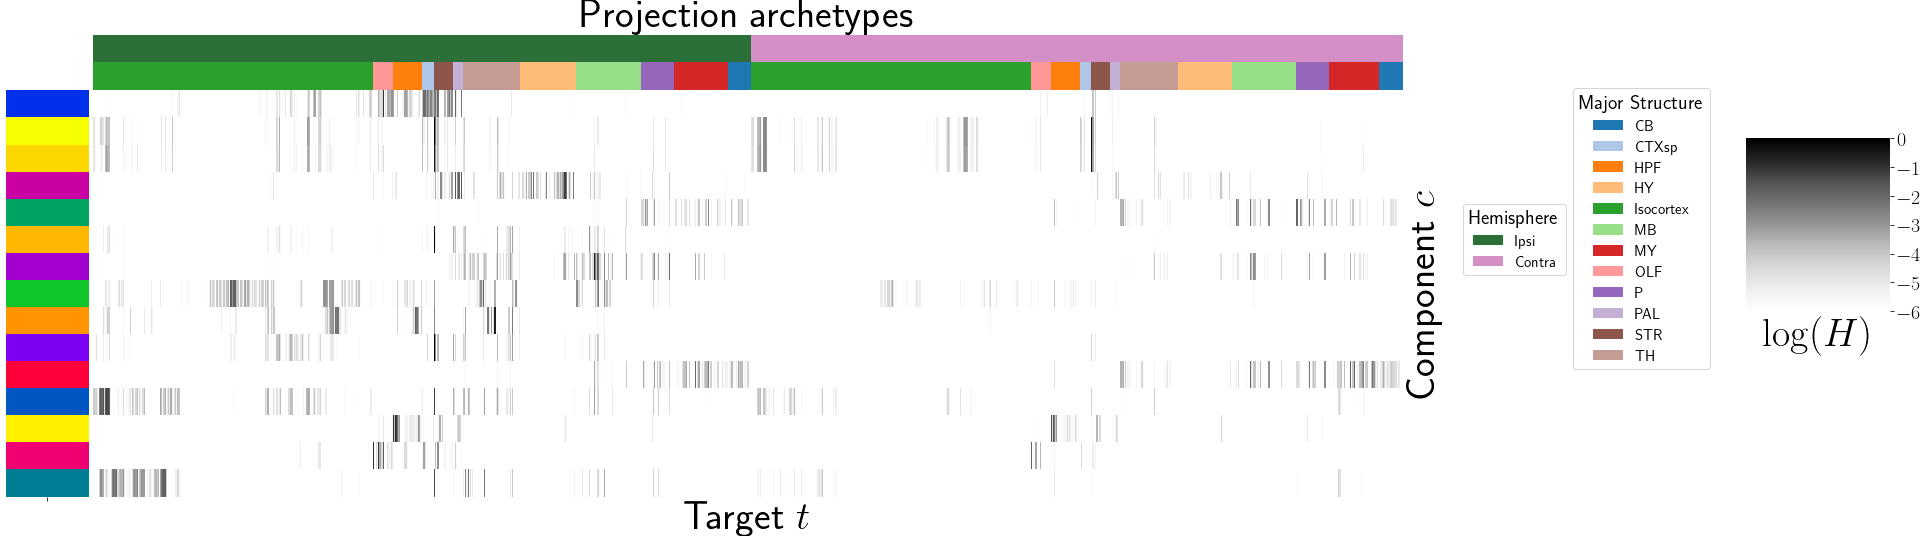
\includegraphics[width = .8 \textwidth]{../../paper/figures/H_wt_0617.png}
\label{fig:H}}
\\
%\subfloat[]{\includegraphics[width = 1.5in]{figs/figsforpres/test_train.png}} &
\subfloat[]{
\includegraphics[width = .3\textwidth]{../../paper/figures/W_wt_0617.png}
\label{fig:W}
}
\end{tabular}
\caption{Non-negative matrix factorization results $\mathcal C_{wt} = WH$ for $q = 15$ components.
\ref{fig:H} Latent space coordinates $H$ of $\mathcal C$.
Target major structure and hemisphere are plotted.
\ref{fig:W} Loading matrix $W$.
Source major structure and layer are plotted.
}
\label{fig:nmf_results}
\end{figure}

\newpage


%This analysis shows that there are relatively few architypal signals underlying the overall connectome.

%simply exhibit a collection of these patterns using several factorization methods applied to the connectivity matrix $\mathcal C$.

%Association of these patterns with the underlying biological processes is a fundamental goal in neuroscience.
%Since much of the connectivity matrix can be predicted solely based off of location information.  For this reason, we subtract our the simple $\hat f_{d} c(p_1), c(p_2)$ where $\hat f$ is the estimated relation of distance between regional centroids and connectivity strength.

%, which we elucidate through n. First, projection signals cluster by target and by source; we can identify similarly behaving structures and neural targets that tend to co-occur.  Second, the specific cell-types targeted by the various cre-lines themselves generate a reduced-dimension space. Under the assumption that cell-type determines projection pattern, we can investigate which cell-types are present in which of the projecting structures.

\newpage

\begin{comment}
%}
% \begin{figure}[h]
%     \centering
%     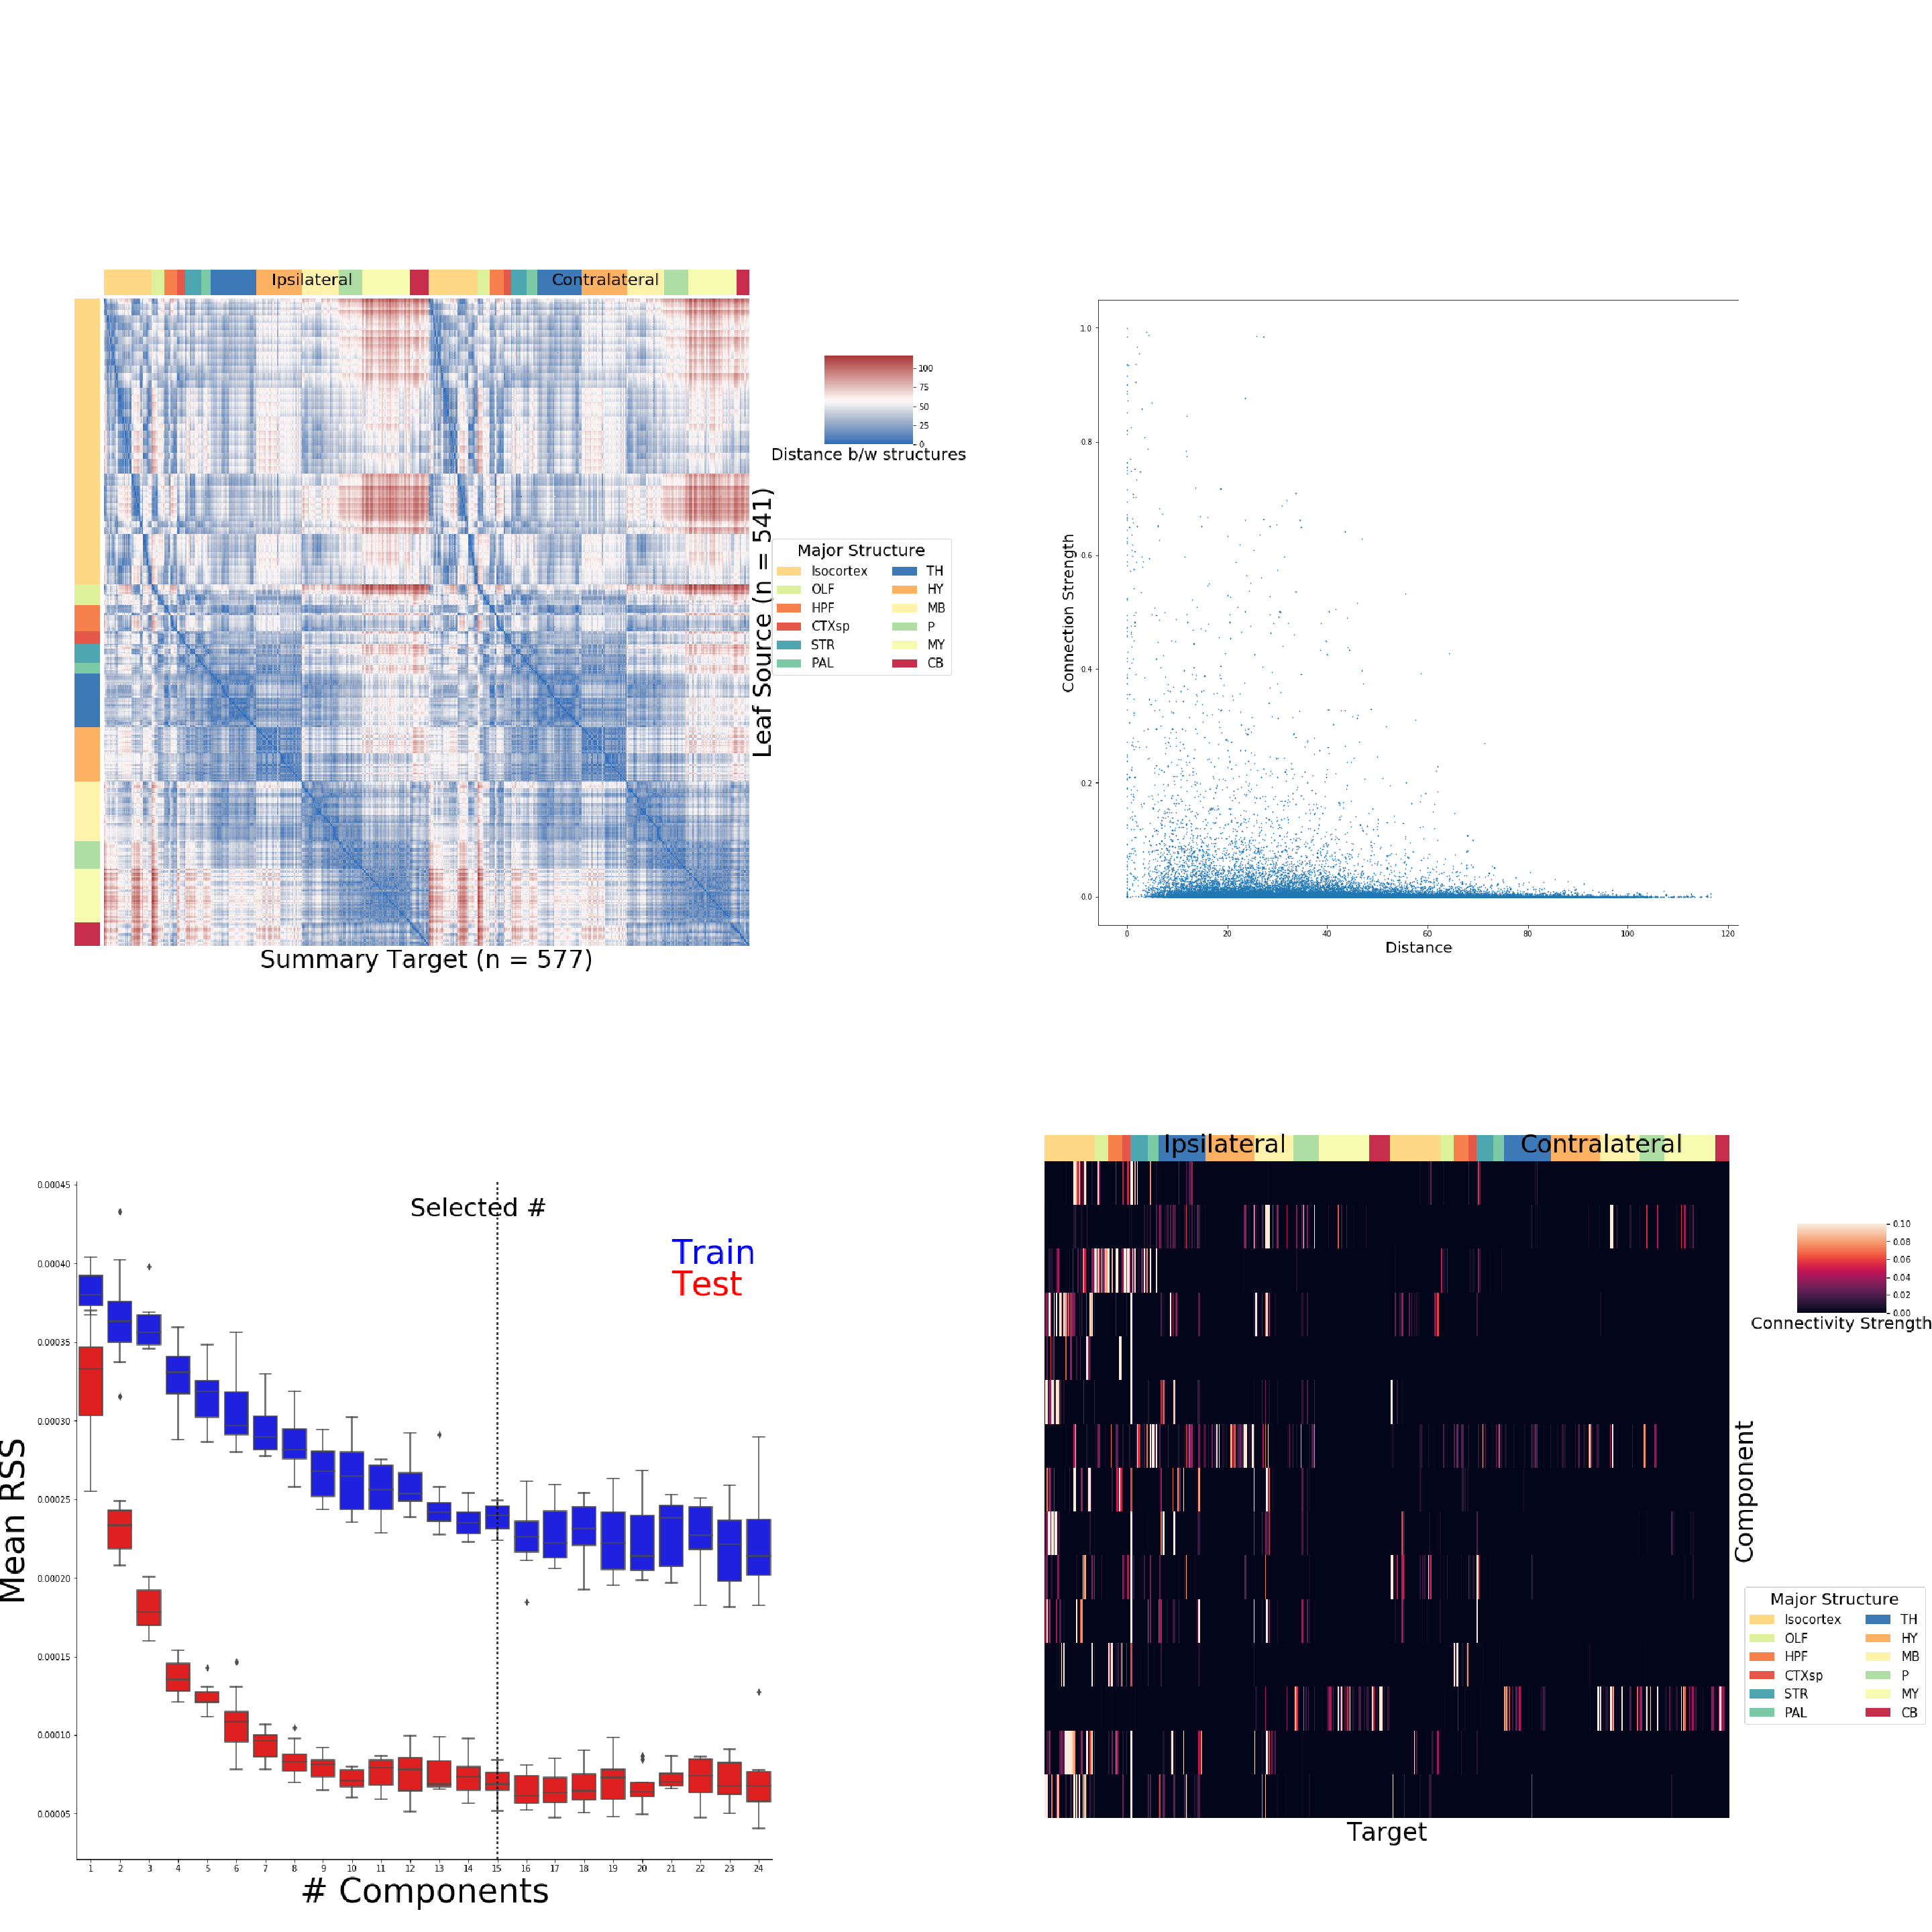
\includegraphics[width = 6in]{figs/Figure5.png}
%     \caption{a) Distances between structures \skcomment{Add units to distance legend}. b) Relation between connectivity strength and distance. c) Train error and test error of non-negative matrix factorization of non-local ($> 1500 \mu m$) connectivities. d) The top $15$ factorization components. \skcomment{Why is compressability so high}}
%     \label{fig:nmf}
% \end{figure}
% \newpage





%Our core model evaluation method is leave-one-out cross validation. This method is robust to the trivial overfitting in Nadaraya-Watson bandwidth selection. We show that incorporation of cre lines improves model performance in the following experimental set-ups. This requires at least two experiments in every experimental division, even in the 2-stage model, since leave-one-out means of each cre line may only be computed for cre-lines which are present at least twice in the leaf. This is the set up for a model trained on all data. However, for alternate models, such as the major-structure divided model from \citet{Knox2019-ot}, the potential evaluation set is larger. In order to compare between methods, we therefore restrict to the smallest set of evaluation indices, which is to say, virus-leaf combinations that are present at least twice.  This means that in some cases, our training set exceeds our evaluation set in size. 

 \begin{comment}
\begin{figure}[H]
\centering
    \subfloat[] {
   % \raisebox{-.5\height}
    \includegraphics[width = \linewidth]{../../analyses/paper/figures/conn_leafs_0617.png}
    } 
    \\
    \vspace{-2cm}
    \subfloat[]{
    \adjustbox{valign=c}{
    \tiny
\begin{tabular}{lrllll}
\toprule
{} &  \#\pbox{20cm} {Ipsilateral \\ Leaf Targets } & \pbox{20cm}{Top \\ Entropy }& Bottom Sparsity & Bottom Entropy & Top Sparsity \\
\midrule
Isocortex &                          51 &          CP &             BAC &            BAC &         ENTl \\
OLF       &                          11 &         TMv &             III &            III &          NaN \\
HPF       &                          15 &          IG &             EPv &             PA &          NaN \\
CTXsp     &                           7 &          TT &              FC &            APr &           TT \\
STR       &                          14 &         RPA &             ISN &            PYR &           TU \\
PAL       &                           9 &          PG &           ACVII &             GR &           MG \\
TH        &                          44 &         NOD &              DN &         SSp-ll &          SCm \\
HY        &                          44 &         CLA &              SH &            LSc &           DG \\
MB        &                          39 &         NDB &            SubG &            SGN &          SUB \\
P         &                          26 &          MT &            Acs5 &            SOC &          NDB \\
MY        &                          43 &          RT &             NaN &             OV &          EPd \\
CB        &                          18 &         ECT &             AOB &            MOB &           GU \\
\bottomrule
\end{tabular}
    }
}
    \subfloat[]{
    \adjustbox{valign=c}{
    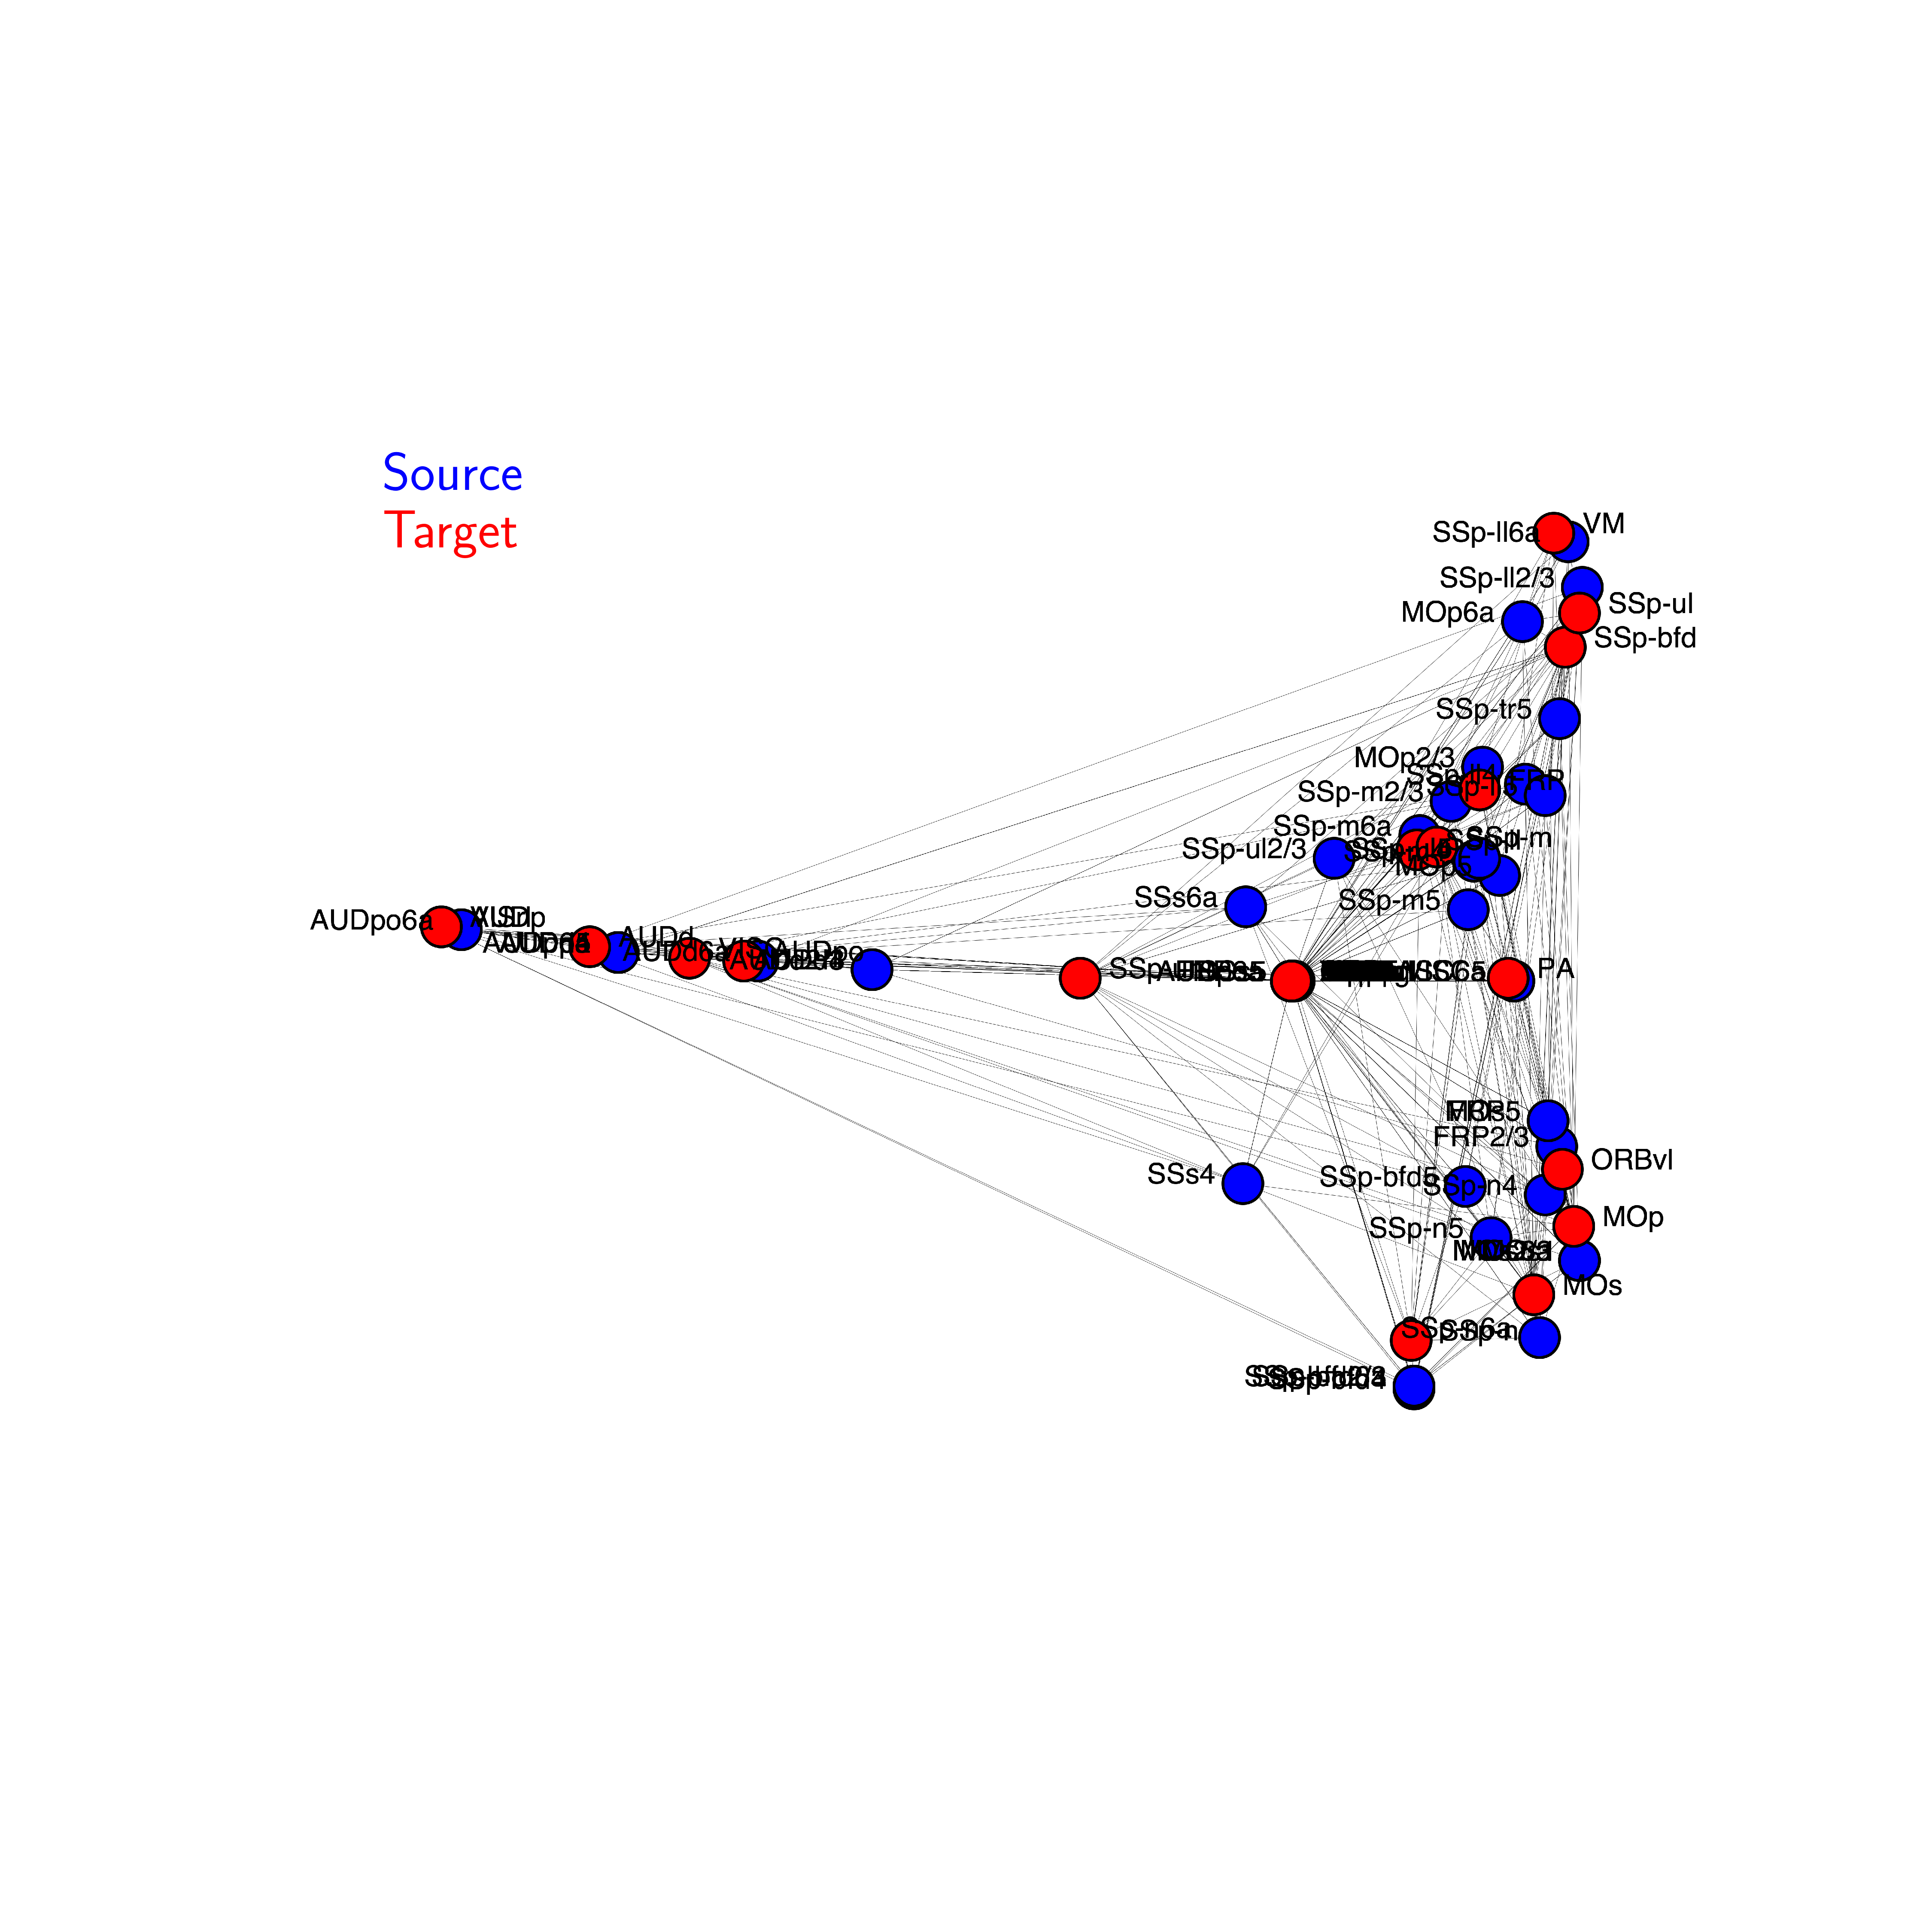
\includegraphics[width = 3in]{figs/st_graph}
    }
    } \\
     \vspace{-4cm}
    \subfloat[]{
    \adjustbox{valign=c}{
    \tiny
    \begin{tabular}{lrllll}
       
\toprule
{} &  \# Ipsilateral Leaf Targets & Top Entropy & Bottom Sparsity & Bottom Entropy & Top Sparsity \\
\midrule
Isocortex &                          51 &          CP &             BAC &            BAC &         ENTl \\
OLF       &                          11 &         TMv &             III &            III &          NaN \\
HPF       &                          15 &          IG &             EPv &             PA &          NaN \\
CTXsp     &                           7 &          TT &              FC &            APr &           TT \\
STR       &                          14 &         RPA &             ISN &            PYR &           TU \\
PAL       &                           9 &          PG &           ACVII &             GR &           MG \\
TH        &                          44 &         NOD &              DN &         SSp-ll &          SCm \\
HY        &                          44 &         CLA &              SH &            LSc &           DG \\
MB        &                          39 &         NDB &            SubG &            SGN &          SUB \\
P         &                          26 &          MT &            Acs5 &            SOC &          NDB \\
MY        &                          43 &          RT &             NaN &             OV &          EPd \\
CB        &                          18 &         ECT &             AOB &            MOB &           GU \\
\bottomrule
\end{tabular}
}
}
\vspace{-4cm}
    \subfloat[]{
    \adjustbox{valign=c}{
    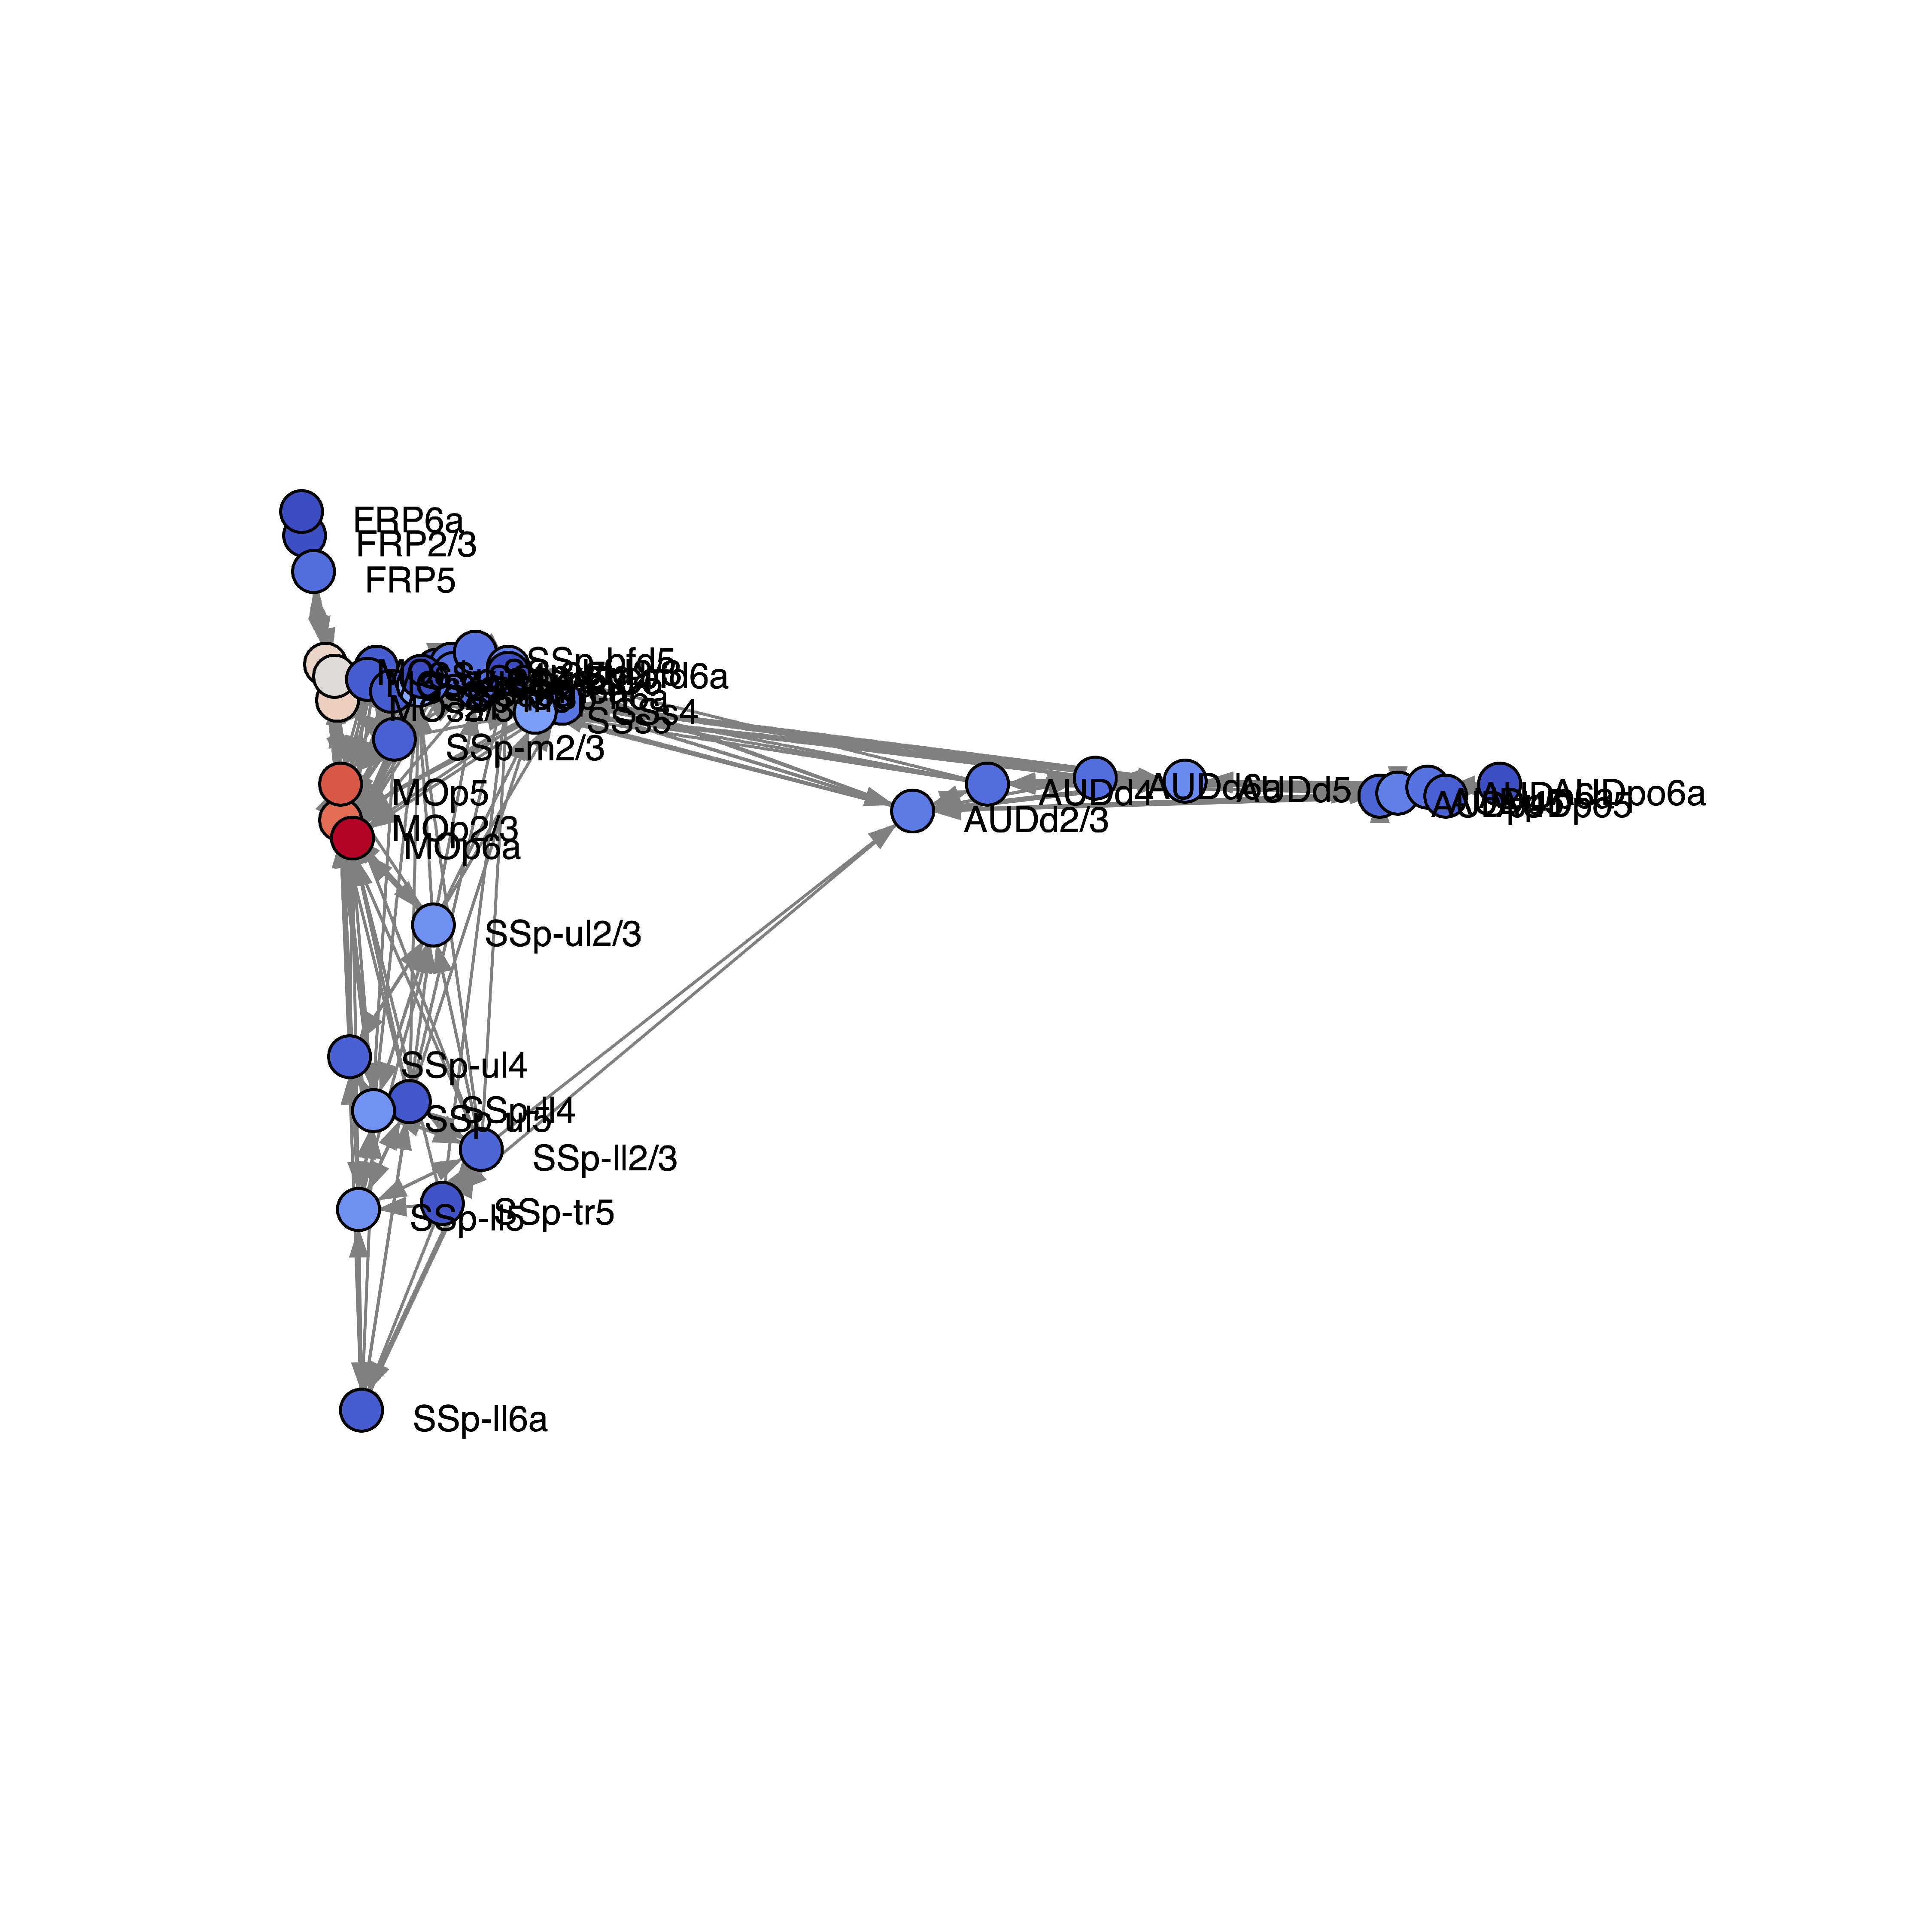
\includegraphics[width = 3in]{figs/page_graph}
    }
    }
\end{figure}
\end{comment}

%\begin{figure}[p]
%    \centering
%    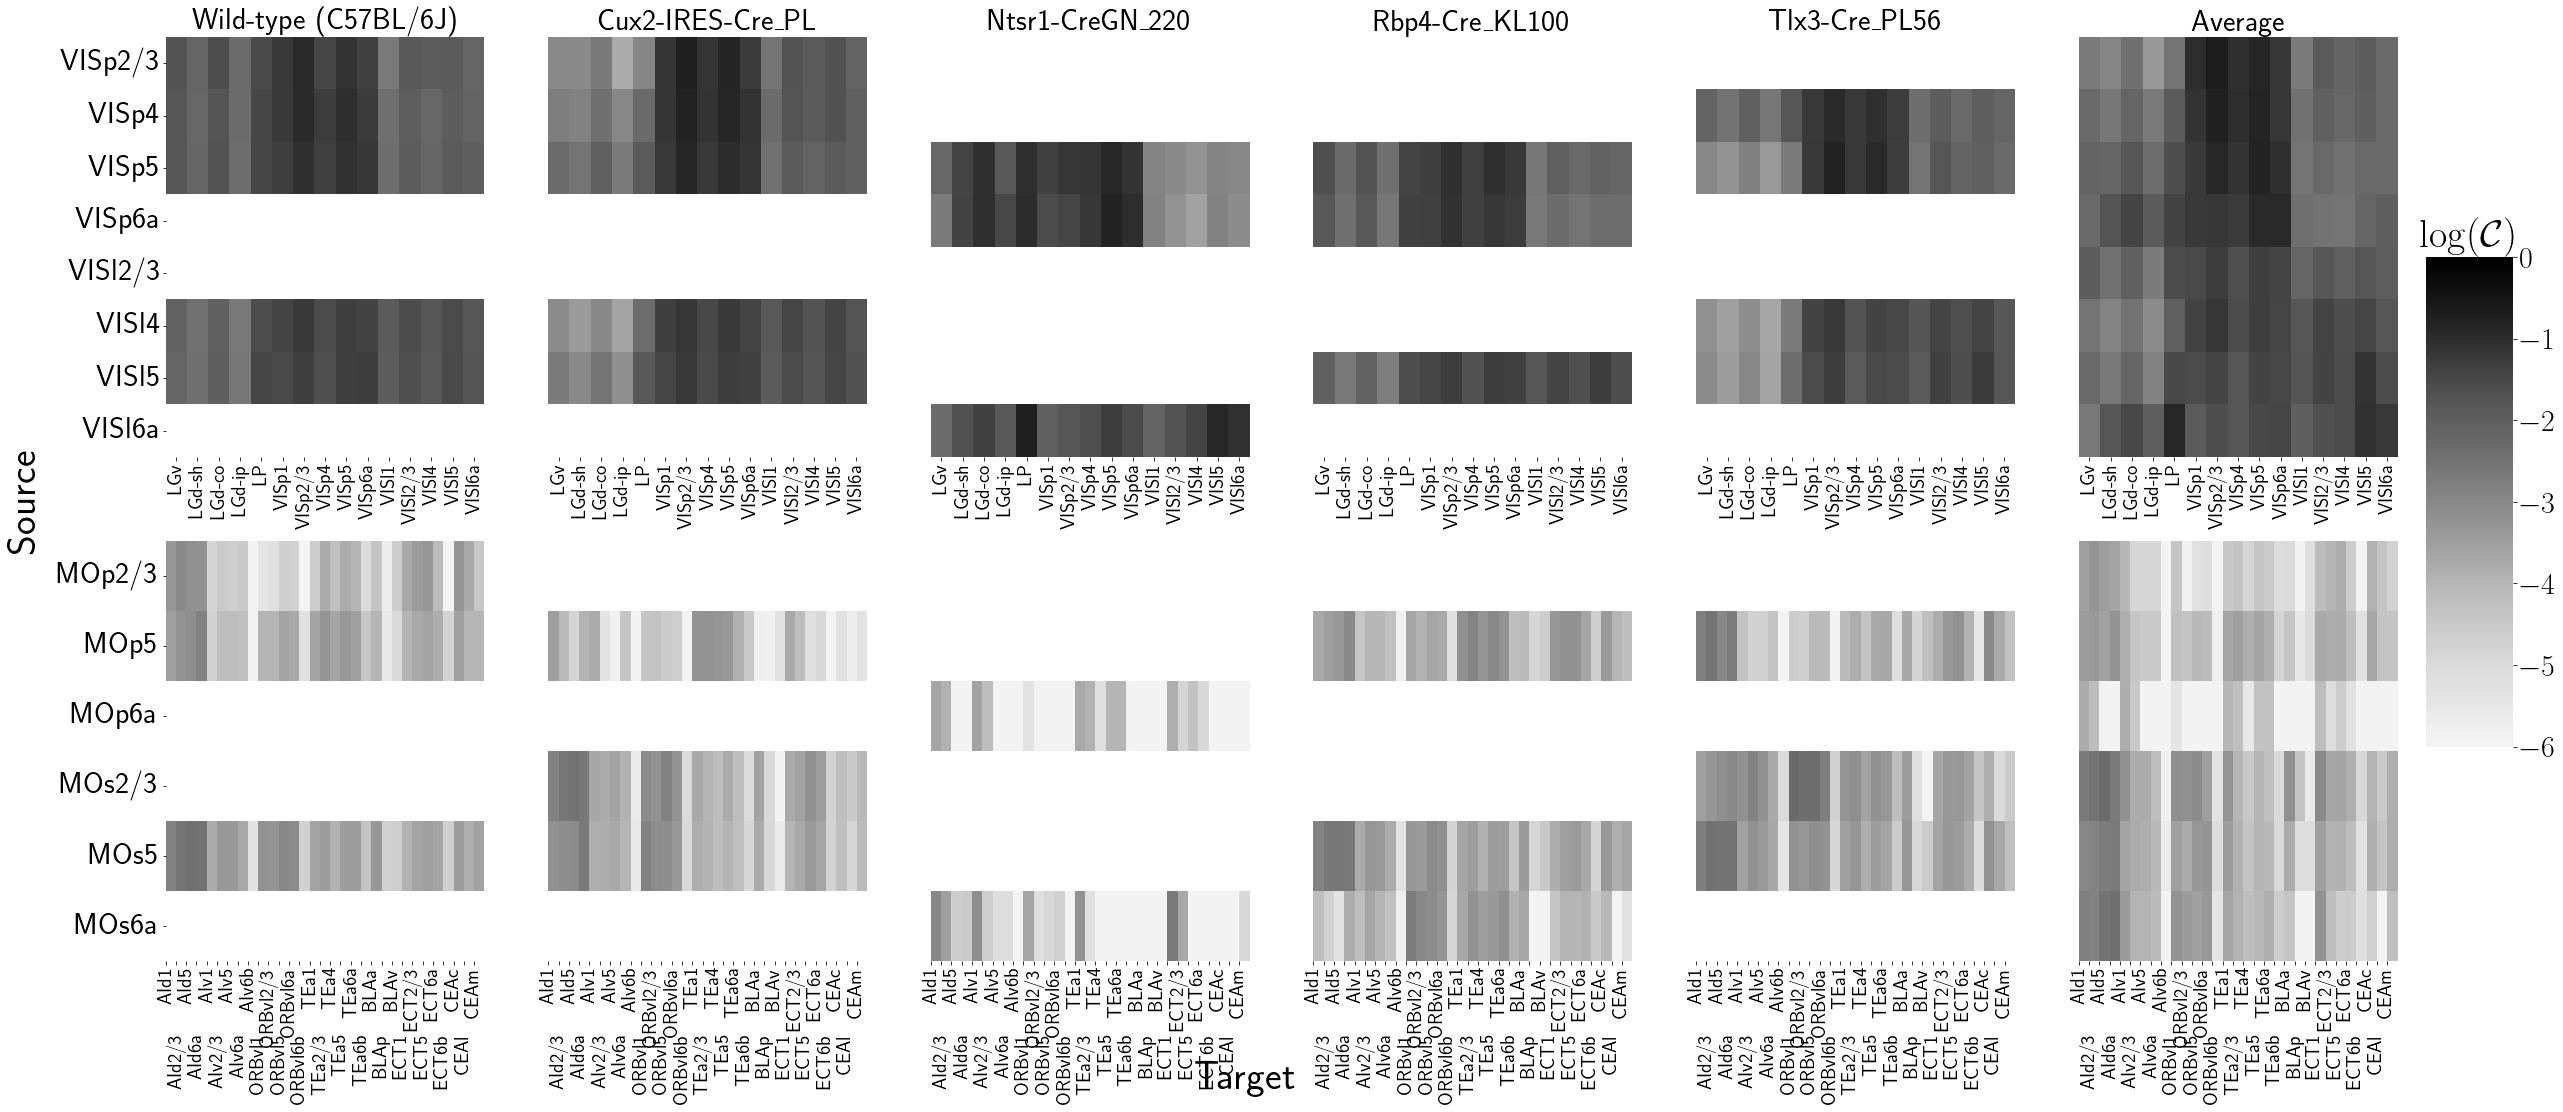
\includegraphics[width = 18cm]{figs/visp_mo.png}
%    \caption{Cre-line specific connectivity matrices for a selection of sources and targets are displayed as heatmaps. Sources without a injection of that cre-type are blank.}
%    \label{fig:my_label}
%\end{figure}


